\documentclass[12pt,a4paper,oneside,openright]{book}
\usepackage{packages} % inserisce tutti le macro necessarie per il
                        % funzionamento
\usepackage{frontesp} % modificare questo file per i diplomi e se si ha
                        % un solo correlatore
\usepackage{setspace}
\usepackage[utf8]{inputenc}
\usepackage[italian]{babel}
\usepackage{graphicx}
\usepackage{booktabs}
\usepackage[showframe]{geometry}

\setstretch{1.3}  %interlinea, mettere 1 per singola da usarsi per le bozze!!!

\begin{document}

\setlength{\headsep}{1pt}
\begin{figure}
	\centering
	
\includegraphics[width=6cm]{images/logo.png}
\end{figure}
\hfill

\title{Titolo tesi italiano}
\hfill
\providecommand{\entitle}{Titolo tesi inglese}

\providecommand{\autore}{Nome candidato}                        %candidato
\providecommand{\matricola}{matricola}
\providecommand{\principaladviser}{Prof.~Ipse Dixit}  %relatore
\providecommand{\firstreader}{Prof.~Ipse Dixit}            %correlatore
%\providecommand{\secondreader}{Chiar.mo~Prof. R. SEMPRONIO}   %correlatore
\providecommand{\annoacc}{2017/18}
%\providecommand{\tipo}{TRIENNALE} % corso di laurea in ??
\providecommand{\corso}{INFORMATICA, ELETTRONICA E DELLE TELECOMUNICAZIONI} % corso di laurea in ??

% genera la prima pagina

\titlep

% indica l'inizio della parte introduttiva
\frontmatter

   \vspace*{10pc}
\thispagestyle{empty}
\begin{flushright}
\sl

Ringrazio IMP Lab per il template... :)

\end{flushright}
\par\vfill\par

   \tableofcontents
   \listoffigures
   \listoftables
%   \listofalgorithms

\clearpage

% indica l'inizio della parte centrale
\mainmatter
 %\input{abstract}
 \chapter*{Introduzione}
\markboth{Introduzione}{Introduzione}
\addcontentsline{toc}{chapter}{Introduzione}

Introduzione della tesi. % attenzione! guardare introd.tex per vedere come e' fatto
 \chapter{Teoria}
\label{teoria}


Capitolo uno:
esempio di bibliografia \cite{2015arXiv150200046K}, un esempio di figura \ref{figure:test inserimento} e un esempio di tabella \ref{table:esempio_tabella}.

\begin{figure}
	\centering
	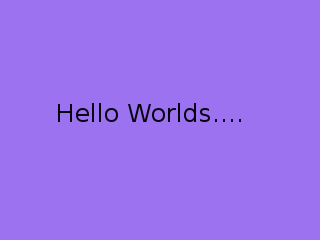
\includegraphics[width=8cm]{images/example.png}
	\caption{Test inserimento immagini}
	\label{figure:test inserimento}
\end{figure}

\begin{table}[!htbp]
	\centering
	\begin{tabular}{l|l}
		\toprule
		Colonna 1 & Colonna 2 \\
		\midrule
		Valore 1 & Valore 2 \\
		Valore 3 & Valore 4 \\
		Valore 5 & Valore 6 \\
		\bottomrule
	\end{tabular}
	\caption{Descrizione della tabella}
	\label{table:esempio_tabella}
\end{table}
 \chapter{Dettagli implementativi}
 \chapter{Esperimenti e risultati}
 \chapter{Ottimizzazioni e risultati}
 \chapter{Conclusioni e sviluppi futuri}
% altri capitoli...

% da qui in poi \chapter genera un'appendice
\appendix
\renewcommand{\chaptermark}[1]{\markboth{{\appendixname}\ \thechapter.\hspace{1em}#1}{}}

\clearpage
\addcontentsline{toc}{chapter}{Bibliografia}
\bibliography{citazioni}
%\bibliographystyle{abbrv}
\bibliographystyle{ieeetr}


%\cfoot{\emph{Finito di stampare il \today\/ utilizzando \LaTeXe}}
\end{document}
